\documentclass{article}

\usepackage[a4paper]{geometry}
\usepackage[ngerman]{babel}
\usepackage[utf8]{inputenc}
\usepackage[T1]{fontenc}
\usepackage[table]{xcolor}
\usepackage{graphicx}

\graphicspath{ {./images/} }

\renewcommand\thesubsection{\alph{subsection})}

\begin{document}

\begin{titlepage}
	\begin{flushleft}
		TH Brandenburg \\
		Online Studiengang Medieninformatik \\
		Fachbereich Informatik und Medien \\
		Kommunikationsnetze 1 \\
		Prof. Dr.-Ing. habil. Michael Syrjakow
	\end{flushleft}

	\vfill

	\begin{center}
		\Large{Einsendeaufgabe 2}\\[0.5em]
		\large{Sommersemester 2021}\\[0.25em]
		\large{Abgabetermin 21.05.2021}
	\end{center}

	\vfill

	\begin{flushright}
		Maximilian Schulke \\
		Matrikel-Nr. 20215853
	\end{flushright}
\end{titlepage}

\newpage

\section*{Aufgabenstellung}

Eine Firma hat das Class C Netz 198.2.11.0 zugewiesen bekommen. Host A, Host B, Host C, R1 und R2 gehören
einer Firma, R ist ein Router im Internet. Die Firma benötigt drei Subnetze, wobei in den Subnetzen 2 und
3 jeweils nicht mehr als 10 Rechner angeschlossen werden sollen, alle anderen Rechner werden im Netz 1
angeschlossen.

\begin{figure}[ht]
	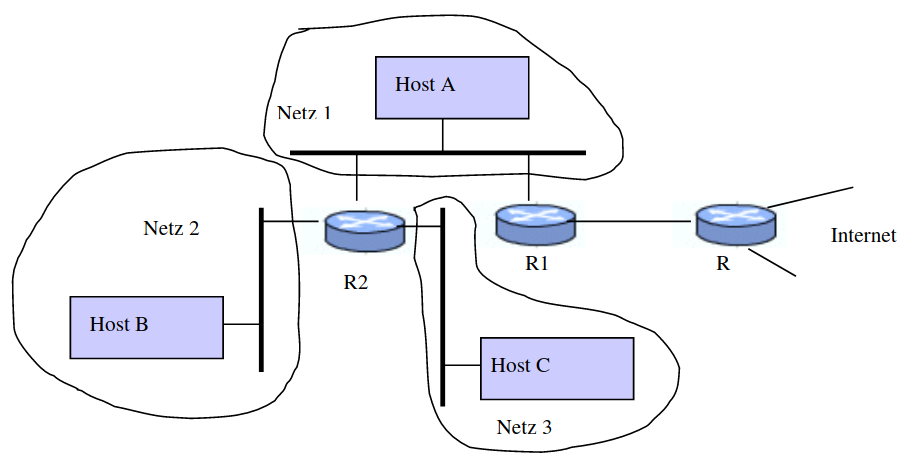
\includegraphics[width=0.75\textwidth]{plain}
	\centering
	\caption{Netzwerk}
\end{figure}

\section*{Lösung}

\subsection{Legen Sie die Adressen der Subnetze und deren Subnetzmasken bzw. Präfixe fest.}

\begin{tabular}{|c|c|c|}
	\hline
	Netz & Adresse        & Subnetzmaske    \\
	\hline
	1    & 198.2.11.0/24  & 255.255.255.0   \\
	\hline
	2    & 198.2.11.16/28 & 255.255.255.240 \\
	\hline
	3    & 198.2.11.32/28 & 255.255.255.240 \\
	\hline
\end{tabular}

\subsection{Legen Sie die Adressen in Netz 1 des Hosts A und der Router-Interfaces von R1 und R2 fest.}

\begin{tabular}{|c|c|}
	\hline
	Gerät  & Adresse       \\
	\hline
	R1     & 198.2.11.1/24 \\
	\hline
	R2     & 198.2.11.2/24 \\
	\hline
	Host A & 198.2.11.3/24 \\
	\hline
\end{tabular}

\subsection{Legen Sie die Adressen in Netz 2 des Hosts B und des Router-Interfaces von R2 fest.}

\begin{tabular}{|c|c|}
	\hline
	Gerät  & Adresse        \\
	\hline
	R2     & 198.2.11.17/28 \\
	\hline
	Host B & 198.2.11.18/28 \\
	\hline
\end{tabular}

\subsection{Legen Sie die Adressen in Netz 3 des Hosts C und des Router-Interfaces von R2 fest.}

\begin{tabular}{|c|c|}
	\hline
	Gerät  & Adresse        \\
	\hline
	R2     & 198.2.11.33/28 \\
	\hline
	Host C & 198.2.11.34/28 \\
	\hline
\end{tabular}

\subsection{Tragen Sie alle Adressen in die Zeichnung ein.}

\subsection{Legen Sie die Einträge in den Routing-Tabellen für Host A, Host B, Host C sowie R1 und R2 so
fest, dass von allen Rechnern aus das Internet sowie die Subnetze erreichbar sind.}

\vspace{1em}

\subsubsection*{R1}

\begin{tabular}{|c|c|}
	\hline
	default        & <Adresse von R> \\
	\hline
	198.2.11.16/28 & 198.2.11.2/24   \\
	\hline
	198.2.11.32/28 & 198.2.11.2/24   \\
	\hline
\end{tabular}

\subsubsection*{R2}

\begin{tabular}{|c|c|}
	\hline
	default        & 198.2.11.1/24 \\
	\hline
\end{tabular}

\subsubsection*{Host A}

\begin{tabular}{|c|c|}
	\hline
	default        & 198.2.11.1/24 \\
	\hline
	198.2.11.16/28 & 198.2.11.2/24 \\
	\hline
	198.2.11.32/28 & 198.2.11.2/24 \\
	\hline
\end{tabular}

\subsubsection*{Host B}

\begin{tabular}{|c|c|}
	\hline
	default & 198.2.11.17/28 \\
	\hline
\end{tabular}

\subsubsection*{Host C}

\begin{tabular}{|c|c|}
	\hline
	default & 198.2.11.33/28 \\
	\hline
\end{tabular}

\subsection{Welchen Eintrag braucht ein Router im Internet, damit das Netz und die Subnetze der Firma erreicht
werden können? Wie sieht die Subnetzmaske bzw. das Präfix aus?}

Jedes Paket was in das Firmennetz verschickt werden soll muss immer zu erst an R1 geroutet werden, da nur R1 die
interne Netzstruktur kennt. Daher muss der folgende Eintrag vorhanden sein:

\vspace{1em}

\begin{tabular}{|c|c|}
	\hline
	198.2.11.0/24 & 198.2.11.1/24 \\
	\hline
\end{tabular}

\end{document}

